\label{sec-theory}

\subsection{ECG, morfologia e segmentação}

Um batimento ECG típico apresenta onda P, complexo QRS e onda T. A anotação de
batimento na MIT-BIH fornece uma referência temporal associada ao evento
cardíaco, usada no protocolo como centro da janela de extração. A
Figura~\ref{fig-ecg-schema} mostra as regiões fisiológicas aproximadas usadas
para organizar as features locais.

\begin{figure}[!htbp]
  \centering
  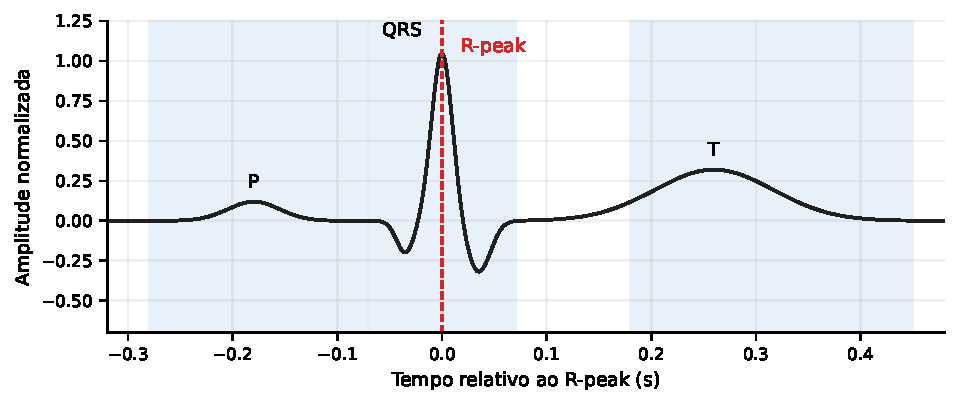
\includegraphics[width=0.95\linewidth]{figures/fig_ecg_waves_schema.pdf}
  \caption{Batimento ECG com onda P, complexo QRS, onda T, R-peak e janelas
  aproximadas usadas na extração de features.}
  \label{fig-ecg-schema}
\end{figure}

\subsection{Filtragem FIR}

Registros ambulatoriais de ECG podem conter deriva de linha de base,
interferência de rede e ruído de alta frequência. A literatura de
monitoramento e detecção de QRS sustenta o uso de bandas reduzidas quando a
pergunta depende sobretudo da morfologia do batimento e da localização do
complexo QRS. Thakor et al. mostraram que um passa-faixa centrado próximo de
17 Hz melhora a razão sinal-ruído do QRS em relação a T, ruído muscular e
interferência de rede \citep{thakor1984qrs}. Elgendi et al. analisaram sinais
da MIT-BIH e indicaram que a faixa de 0,5 a 40 Hz preserva componentes centrais
do QRS em aplicações de detecção e processamento eficiente
\citep{elgendi2017efficient}. O protocolo usa, portanto, uma cadeia FIR
passa-faixa de 0,5 a 40 Hz com janela de Hamming e aplicação forward-backward
em fase zero. O rejeita-faixa em 60 Hz não é mantido, pois a própria etapa
passa-baixa já remove a interferência de rede fora da banda preservada. O ganho
dessa etapa é medido pela comparação entre \texttt{A0 raw} e
\texttt{A1 filtered}, sem pressupor melhora automática na detecção.

\subsection{STFT e filtros de Gabor}

Estruturas do ECG ocupam escalas temporais distintas. O complexo QRS é curto e
concentra componentes relativamente rápidas, enquanto P e T tendem a aparecer
em janelas mais largas e suaves. A STFT resume energia local em janelas curtas;
filtros de Gabor 1D representam o sinal por átomos localizados no tempo e na
frequência \citep{gabor1946theory}. Essa família já foi usada para extrair
features de ECG em combinação com STFT e modelos gaussianos
\citep{lee2012gabor}, e transformadas de Gabor de Q constante aparecem em
representações tempo-frequência recentes para diagnóstico automático em ECG
\citep{eltrass2021cqgabor}. Para um sinal discreto \(x[n]\), a STFT pode ser
escrita como

\[
X(m, \omega)=\sum_n x[n]w[n-m]e^{-j\omega n},
\]

em que \(w\) define a janela temporal local. Os filtros de Gabor usados como
features seguem a ideia de uma portadora senoidal modulada por uma envoltória
gaussiana,

\[
g_{f,\sigma}(t)=e^{-t^2/(2\sigma^2)}\cos(2\pi f t).
\]

A entrada das features Gabor apenas em \texttt{A3} isola sua contribuição em
relação a morfologia, RR e espectro. Para evitar uma expansão excessiva da
dimensionalidade, o banco é definido por região fisiológica aproximada. A
janela P usa frequência central de 7 Hz, o QRS usa 15 Hz e a janela T usa
5 Hz, com três ciclos no envelope gaussiano. A escolha acompanha a leitura
fisiológica de P e T como eventos mais lentos e largos que o QRS, enquanto a
frequência do QRS permanece próxima da região de maior separação espectral
descrita por Thakor et al. \citep{thakor1984qrs}. As respostas real e
imaginária são combinadas em magnitude, reduzindo a dependência da fase local
do complexo.

\subsection{Detecção one-class}

One-Class SVM estima uma região de suporte para dados normais
\citep{scholkopf2001support}. A formulação primal busca separar os exemplos
normais da origem no espaço de features,

\[
\min_{w,\rho,\xi}\frac{1}{2}\|w\|^2+\frac{1}{\nu n}\sum_i \xi_i-\rho
\quad
\text{sujeito a}
\quad
w^\top\phi(x_i)\geq\rho-\xi_i,\ \xi_i\geq0.
\]

Isolation Forest atribui maior anomalia a pontos isolados por menos
particionamentos aleatórios \citep{liu2008isolation}. O escore depende do
comprimento esperado do caminho \(E[h(x)]\) nas árvores,

\[
s(x,n)=2^{-E[h(x)]/c(n)}.
\]

Local Outlier Factor compara a densidade de uma amostra com a densidade de seus
vizinhos \citep{breunig2000lof}. A densidade de alcançabilidade local e o fator
LOF podem ser resumidos por

\[
\operatorname{lrd}_k(p)=
\left(
\frac{1}{|N_k(p)|}
\sum_{o\in N_k(p)}\operatorname{reachdist}_k(p,o)
\right)^{-1}
\]

e

\[
\operatorname{LOF}_k(p)=
\frac{1}{|N_k(p)|}
\sum_{o\in N_k(p)}
\frac{\operatorname{lrd}_k(o)}{\operatorname{lrd}_k(p)}.
\]

No scikit-learn, o uso de LOF para novelty detection requer
\texttt{novelty=True} e avaliação em dados diferentes dos dados usados no
ajuste \citep{sklearnNovelty}.

\subsection{Custo computacional e inferência}

A comparação de detectores também depende do custo necessário para transformar
um batimento em decisão. Pimentel et al. tratam eficiência como parte da
aplicabilidade de métodos de novelty detection, especialmente quando o modelo de
normalidade precisa operar sobre muitos exemplos de teste
\citep{pimentel2014novelty}. Isolation Forest foi proposto com complexidade
linear e baixo uso de memória por subamostragem, enquanto LOF depende de
consultas a vizinhos e pode ficar mais sensível ao crescimento dimensional
\citep{liu2008isolation,breunig2000lof}. Em aplicações de monitoramento
contínuo, a literatura de edge computing motiva processar dados perto da fonte
quando tempo de resposta, energia e transmissão são restrições relevantes
\citep{shi2016edge}.

\subsection{Avaliação inter-paciente e dados desbalanceados}

A separação entre pacientes reduz avaliações otimistas causadas por
similaridade intra-paciente. Por esse motivo, a divisão DS1 e DS2 usada em
estudos com MIT-BIH orienta o protocolo experimental
\citep{mousavi2019inter}. A PR-AUC recebe prioridade narrativa porque anomalias
são minoria e a curva precision-recall responde diretamente à quantidade de
falsos positivos entre os casos sinalizados \citep{davis2006prroc}.
